% Тут используется класс, установленный на сервере Papeeria. На случай, если
% текст понадобится редактировать где-то в другом месте, рядом лежит файл matmex-diploma-custom.cls
% который в момент своего создания был идентичен классу, установленному на сервере.
% Для того, чтобы им воспользоваться, замените matmex-diploma на matmex-diploma-custom
% Если вы работаете исключительно в Papeeria то мы настоятельно рекомендуем пользоваться
% классом matmex-diploma, поскольку он будет автоматически обновляться по мере внесения корректив
%

% По умолчанию используется шрифт 14 размера. Если нужен 12-й шрифт, уберите опцию [14pt]
\documentclass[14pt]{matmex-diploma-custom}
%\documentclass[14pt]{matmex-diploma-custom}

\begin{document}
% Год, город, название университета и факультета предопределены,
% но можно и поменять.
% Если англоязычная титульная страница не нужна, то ее можно просто удалить.
\filltitle{ru}{
    chair              = {Направление Математики и механики\\ Программная инженерия},
    title              = {Цифровая обработка изображений в микроскопии},
    % Здесь указывается тип работы. Возможные значения:
    %   coursework - Курсовая работа
    %   diploma - Диплом специалиста
    %   master - Диплом магистра
    %   bachelor - Диплом бакалавра
    type               = {diploma},
    position           = {студента},
    group              = 471,
    author             = {Кутуев Владимир Александрович},
    supervisorPosition = {доц.,\,к.т.н.},
    supervisor         = {Литвинов Ю.\,В.},
    % reviewerPosition   = {ст. преп.},
    % reviewer           = {Привалов А.\,И.},
    consultPosition   = {ст. преп.},
    consult           = {Кириленко Я.\,А.},
    % chairHeadPosition  = {д.\,ф.-м.\,н., профессор},
    % chairHead          = {Хунта К.\,Х.},
%   university         = {Санкт-Петербургский Государственный Университет},
%   faculty            = {Математико-механический факультет},
%   city               = {Санкт-Петербург},
%   year               = {2013}
}

\maketitle
\tableofcontents
% У введения нет номера главы
\section*{Введение}

С развитием технологий оптической микроскопии стоимость простых микроскопов стала достаточно низкой для массового использования дома и в образовательных учреждениях. Один из главных факторов получения резких изображений --- оптическая система микроскопа, которая непосредственно влияет на его разрешающую. Но улучшение оптики микроскопа связано с материальными затратами. Цифровая обработка позволяет повысить качество получаемых изображений, без замены оптики. Также получить максимально резкое изображение исключительно средствами оптики микроскопа не всегда возможно: у объёмных препаратов при большом увеличении с помощью микроскопа можно сфокусироваться только на ограниченные области исследуемого объекта, рассеянный свет из областей находящихся вне зоны фокуса влечет появление различных артефактов, которые влияют на чёткость изображения. Цифровая обработка позволяет решить эти проблемы.
\par
Изучаемые в микроскопии объекты могут двигаться, поэтому цифровая обработка должна иметь высокую производительность, чтобы обрабатывать видео в реальном времени с низкой задержкой.
\par
За последние несколько лет мобильные платформы приобрели большую популярность, такой вывод можно сделать на основе статистики анализа web-трафика порталом StatCounter~\cite{StatCounter}. Также интерес к мобильным платформам повышает наличие у большинства смартфонов камер, которые можно использовать для захвата изображений с микроскопа. Поэтому разрабатываемое решение должно быть кроссплатформенным и поддерживать как desktop-платформы, так и основные мобильные --- Android и IOS.

% [Одно из решений - цифровая обработка, хочется обрабатывать видео, учитывая современные тенденции надо проектировать под мобильники (есть камера)]
% [Что-то сказать о интересе обрабатывать видео] [Сказать о популярности телефонов] []
% Одно из решений этой проблемы --- захват видео с микроскопа с помощью смартфона и его обработка для получения чёткого изображения образца. Для этого было решено создать кроссплатформенную библиотеку алгоритмов обработки изображений, которая позволит исправить недостатки изображений, получаемых с оптического микроскопа. 

\section{Постановка задачи}
Цель работы --- разработать кроссплатформенную библиотеку для обработки набора кадров, снятых с использованием оптического микроскопа, которая позволит получать изображение более высокого качества. Также библиотека должна быть расширяемой для внедрения других алгоритмов улучшения получаемого изображения. Важно, чтобы решение работало быстро, сохраняя качество, удовлетворяющее человека. Для достижения цели были поставлены следующие задачи:
\begin{enumerate}
    \item Реализовать систему для визуального сравнения результатов работы алгоритмов обработки набора кадров. 
    \item Провести опрос, какие из алгоритмов выполняют задачу лучше.
    \item Создать прототип для замера скорости работы алгоритмов.
    \item Реализовать кроссплатформенную мобильную библиотеку.
    \item Настроить автоматическую сборку платформно-ориентированных библиотек.
    \item Настроить автоматическое интеграционное тестирование.
\end{enumerate}


\section{Focus stacking(focal stacking)}
Для получения резкого изображения плоского препарата достаточно подобрать расстояние фокусировки, при котором всё изображение попадает в фокус. Однако сделать это с объёмными объектами нельзя. Глубина резкости микроскопа ограничена, и сфокусированными получаются только определённые области препарата. Для решения этой проблемы применяется техника focus stacking: производится захват серии изображений при разных уровнях фокуса, затем для каждого изображения определяются наиболее сфокусированные участки. Из них формируется изображение, в котором все области попадают в фокус (рис.\ref{focus_stacking1}).

\begin{figure}[h]
    \centering
    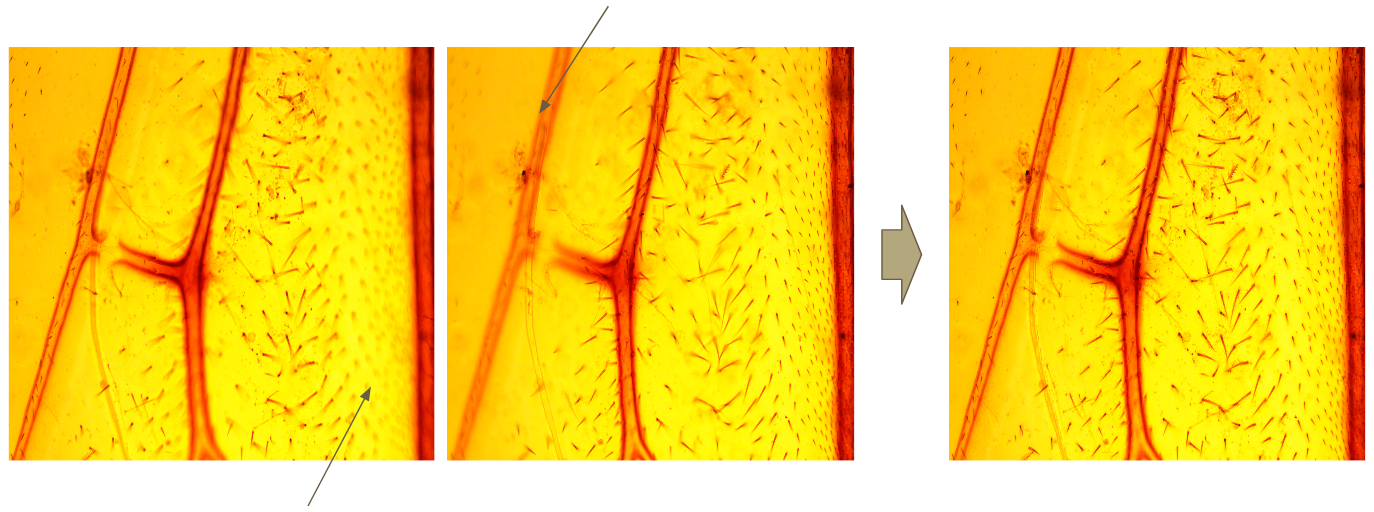
\includegraphics[width=1.0\textwidth]{figures/fs1.png}
    \caption{Focus stacking}
    \label{focus_stacking1}
\end{figure}

\section{Операторы фокусной меры}
Так как было выявлено требование высокому быстродействию обработки серии изображений, то необходимо отбирать наиболее сфокусированных изображений, чтобы сократить время алгоритмов focus stacking и уменьшить количества шума в итоговом изображении. Для определения четкости изображения используются специальные операторы фокусной меры (Objective functions). Они делятся на несколько групп:
\begin{itemize}
    \item Основанные на градиенте
    \item Основанные на операторе Лапласа
    \item Основанные на вейвлет преобразованиях
    \item Статистические
    \item Смешанные
\end{itemize}

Подробный обзор таких операторов приведён в статье "Analysis of focus measure operators for shape-from-focus"~\cite{MeasureOperators}. Также в этой публикации проведено сравнение производительности операторов при различных аспектах: зашумлённость изображений, размер окна оператора. 

Использование операторов фокусной меры для автофокуса в микроскопии было изучено в работе "Automated focusing in bright-field microscopy for tuberculosis detection"~\cite{BestOperators}. В этой статье предлагается использовать операторы фокусной меры и выбирать максимум из результатов их применения на кадрах, снятых микроскопом --- самое сфокусированное положение. В данной публикации проведено сравнения операторов фокусной меры по качеству работы, точности и скорости поиска фокуса с их помощью в области микроскопии. На основе исследования сделан вывод: наиболее подходящими операторами в этой области являются: the normalized variance, the Brenner gradient, the sum-modified Laplacian, the energy of the Laplacian, Vollath F4 and Tenengrad operator.

Опираясь на изученные научные статьи, для использования в прототипе было решено выбрать следующие операторы:
\begin{itemize}
    \item Laplacian Variance 
    \item Tenengrad operator
    \item Vollath F4
    \item Modified Laplacian
\end{itemize}
Выбор сделан с учетом необходимости получения высокопроизводительных операторов, приспособленных к работе с изображениями в области микроскопии.

\section{Повышение качества кадров}
\subsection{Удаление пыли}

Используя операторы фокусной меры, можно столкнуться с проблемой наличия пыли или капель на изображениях --- элементов, которые не являются частью изучаемого препарата, однако попадают в кадр. Пыль обычно находится на приборном стекле или линзе микроскопа, поэтому она оказывается в фокусе в те моменты, когда изучаемый объект размыт. В результате возможно ложное определение кадра как сфокусированного. Чтобы решить эту проблему, можно по расфокусированному содержащему пыль изображению создать маску (рис. \ref{dust_map1}), по которой пыль будет удаляться в обрабатываемых изображениях (рис. \ref{dust_filtering1}).

\begin{figure}[h]
    \centering
    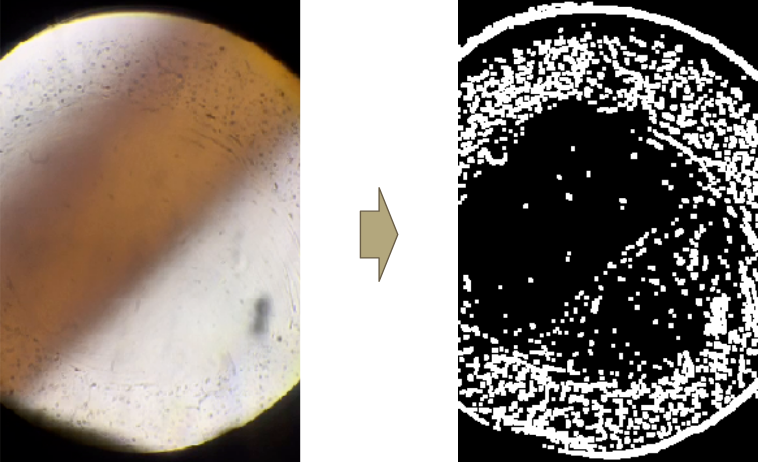
\includegraphics[width=1.0\textwidth]{figures/dust1.png}
    \caption{Создание маски}
    \label{dust_map1}
\end{figure}

\newpage

\begin{figure}[h]
    \centering
    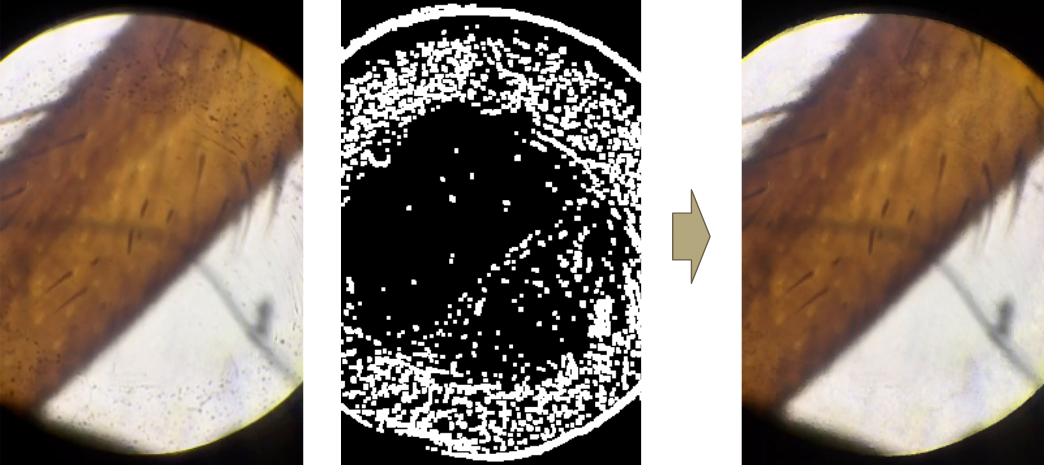
\includegraphics[width=1.0\textwidth]{figures/dust2.png}
    \caption{Удаление пыли}
    \label{dust_filtering1}
\end{figure}


\subsection{Деконволюция}
Рассеянный свет из областей, находящихся вне зоны фокуса, ниже или выше фокальной плоскости, становится причиной появления блеска, искажения и нерезкости при получении изображений. Деконволюция –-- способ обработки изображения, позволяющий избавиться от этих нежелательных эффектов. На Рис.\ref{deconvolution1} представлен результат алгоритма деконволюции "Richardson–Lucy with Total Variation"~\cite{RLTV}. Этот пример показывает, что этот метод позволяет значительно улучшить полученное изображение.

\begin{figure}[h]
    \centering
    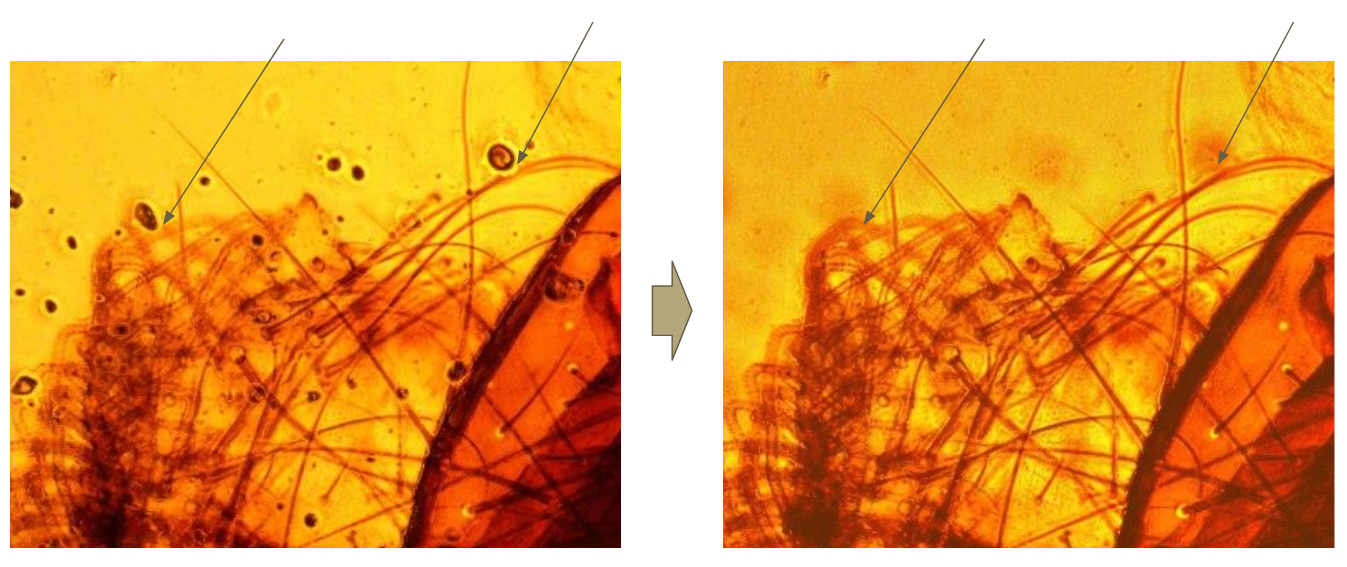
\includegraphics[width=.91\textwidth]{figures/deconvolution1.png}
    \caption{Деконволюция}
    \label{deconvolution1}
\end{figure}

\newpage
Однако деконволюция --- операция, требующая достаточно много времени, поэтому было решено провести исследование, как деконволюция влияет на значение оператора фокусной меры. Рис. \ref{deconvolution2} показывает значение оператора фокусной меры, получаемой на каждом кадре из видео. Можно заметить, что после деконволюции кадры становятся более сфокусированными, но тенденции изменения значения сохраняются на протяжении видео. Дальнейшее исследование должно ответить на вопрос: можно ли отказаться от этой операции на этапе отбора кадров и применять её  только к результату focus stacking.

\begin{figure}[h]
    \centering
    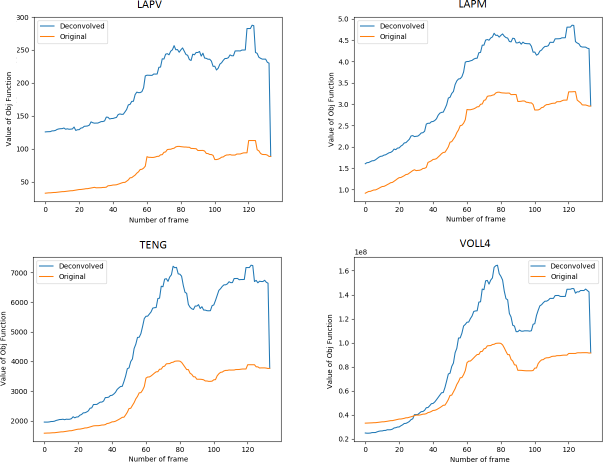
\includegraphics[width=1.0\textwidth]{figures/deconvolution2.png}
    \caption{Значение оператора фокусной меры до и после деконволюции}
    \label{deconvolution2}
\end{figure}


\section{Сравнение результатов работы алгоритмов}

Важная часть работы --- выбор алгоритмов, результат работы которых будет удовлетворительным для человеческого глаза. Отсутствие существенных отличий в результатах нескольких алгоритмов позволит сфокусироваться на более быстрых. Поэтому нужен удобный инструмент для сравнения результатов. Так как целевые устройства --- смартфоны, то этот инструмент должен поддерживать мобильные платформы. Для данных целей разработано web-приложение, удовлетворяющее этим требованиям. На Рис.\ref{comparation1} и Рис.\ref{comparation2} показан его интерфейс. Он разрабатывался с учётом необходимости переключиться между любыми алгоритмами, чтобы сразу увидеть разницу между полученными результатами. Также в этом приложении предусмотрена автоматическая отправка информации, результат какого из алгоритмов понравился опрашиваемому больше.

\begin{figure}[h]
    \centering
    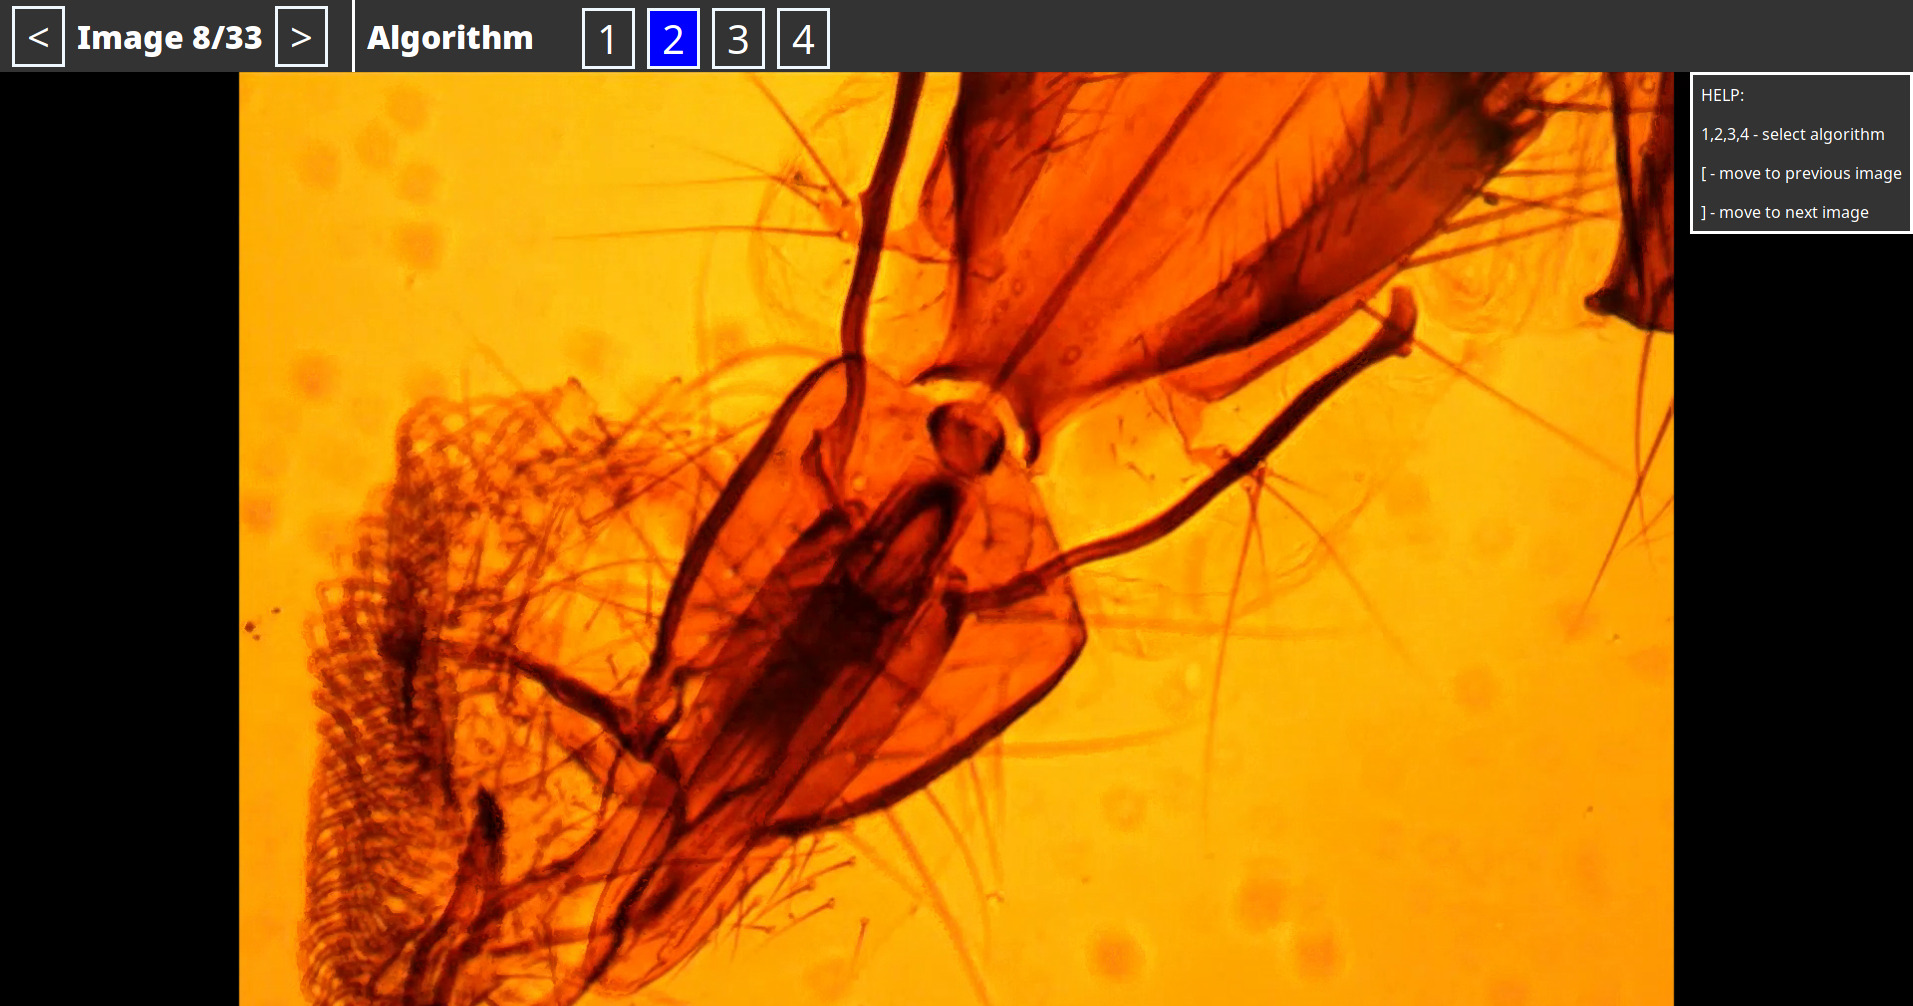
\includegraphics[width=1.0\textwidth]{figures/comparasion1.jpg}
    \caption{Desktop}
    \label{comparation1}
\end{figure}

\newpage

\begin{figure}[h]
    \begin{subfigure}{.25\textwidth}
        \centering
        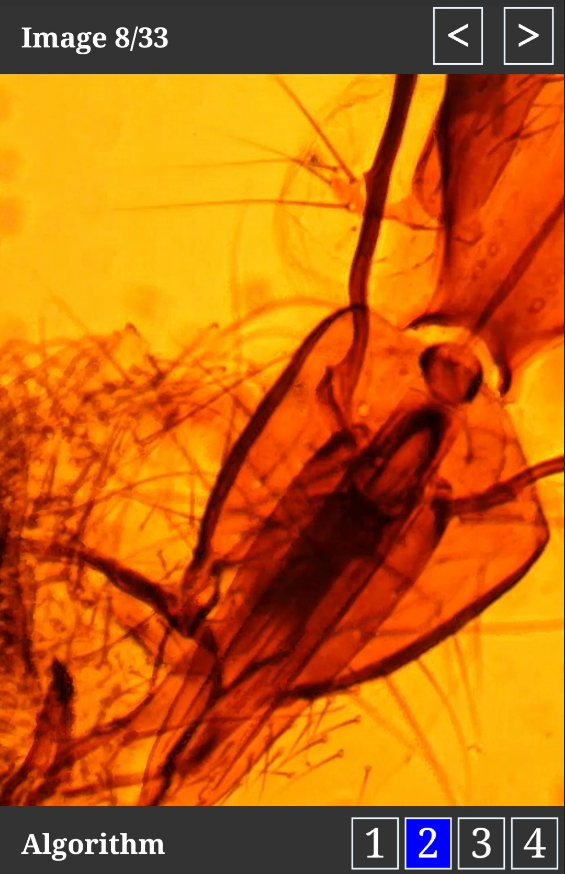
\includegraphics[width=.9\linewidth,height=6cm]{figures/comparasion2.png}
        \caption{Portrait}
        \label{fig:sfig1}
    \end{subfigure}
    \begin{subfigure}{.75\textwidth}
        \centering
        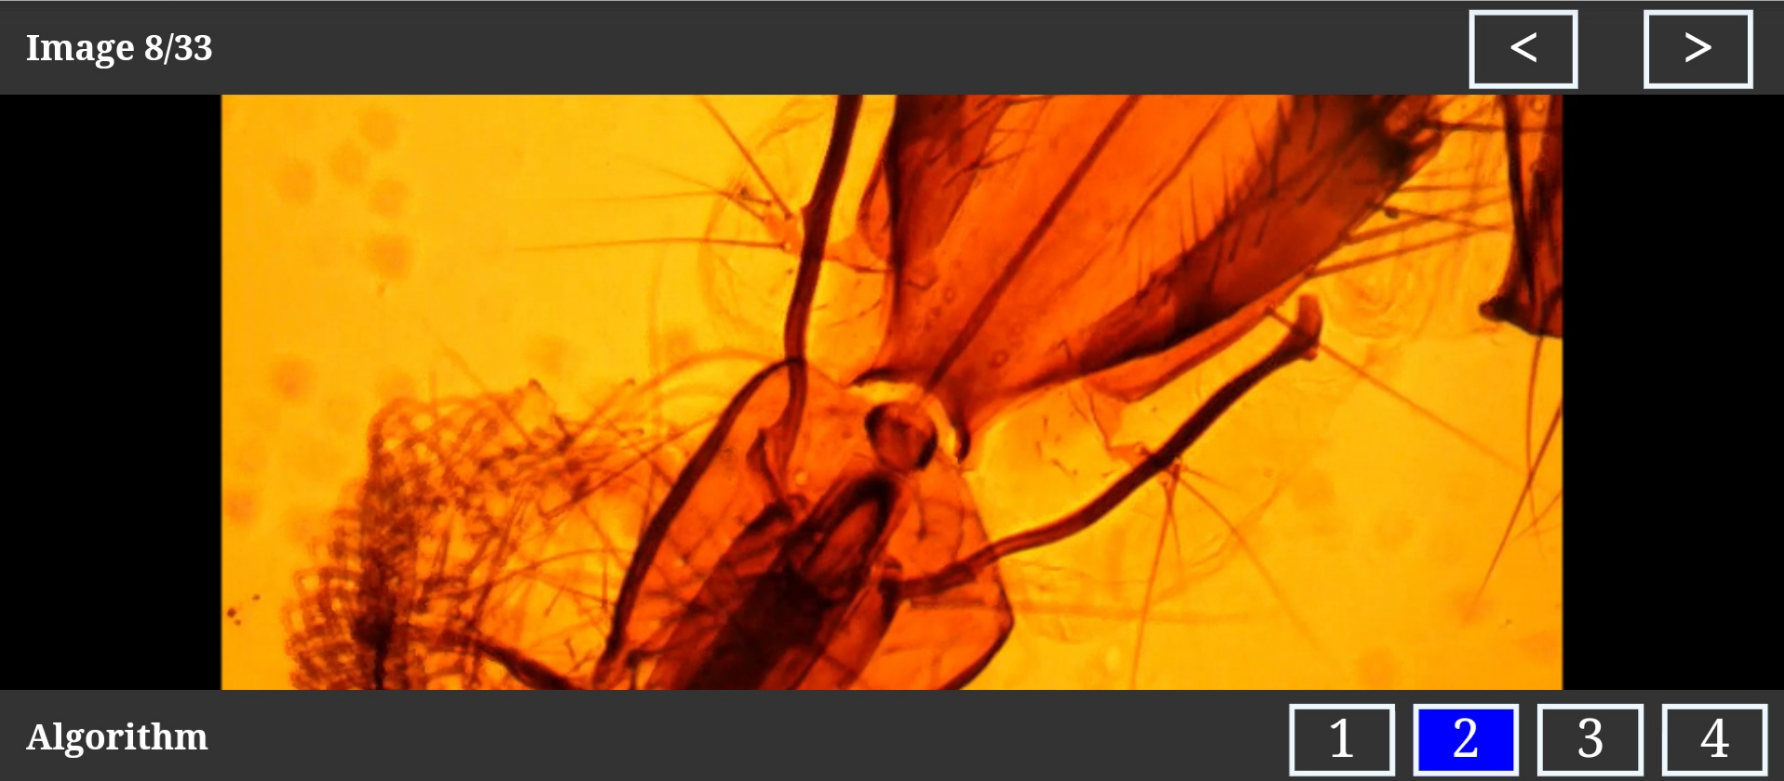
\includegraphics[width=.9\linewidth,height=6cm]{figures/comparasion3.png}
        \caption{Landscape}
        \label{fig:sfig2}
    \end{subfigure}
    \caption{Mobile}
    \label{comparation2}
\end{figure}

\section{Реализация}

Так как важными требованиями к создаваемой библиотеке является быстродействие, то было принято решение реализовывать её на языке программирования C++, а для её использования из-под мобильных платформ воспользоваться инструментом Djinni~\cite{Djinni}. Код на C++ компилируется под нужные платформы, а с помощью Djinni генерируются интерфейсы взаимодействия кода библиотеки с платформенно-ориентированным кодом на Java и Objective-C на Android и IOS. 
\par
В разрабатываемой библиотеке при обработке потока входных кадров и реализации алгоритмов focus stacking и операторов фокусной меры было решено воспользоваться функциональностью, предоставляемой библиотекой OpenCV~\cite{OpenCV}.

% % У заключения нет номера главы
\section*{Заключение}
% В данный момент в библиотеке реализованы:
В ходе работы над проектом были достигнуты следующие результаты:
\begin{enumerate}
    \item Создано web-приложение для визуального сравнения результатов работы алгоритмов. 
    \item В кроссплатформенной библиотеке реализованы:
        \begin{itemize}
            \item оператор фокусной меры Tenengrad;
            \item алгоритм удаления пыли;
            \item алгоритм focus stacking, основанный на одиночных пикселях.
        \end{itemize}
\end{enumerate}

\par
Основные направления дальнейшей работы:
\begin{itemize}
    \item провести опрос, чтобы выявить наиболее подходящие алгоритмы для внедрения в библиотеку
    \item провести замеры скорости работы алгоритмов;
    \item реализовать фильтрацию кадров с одинаковыми областями фокуса;
    \item реализовать выбранные алгоритмы focus stacking;
    \item реализовать выбранные операторы фокусной меры;
    \item реализовать алгоритм деконволюции;
    \item настроить автоматическое интеграционное тестирование;
    \item настроить автоматическую сборку платформно-ориентированных.
\end{itemize}

\setmonofont[Mapping=tex-text]{CMU Typewriter Text}
\bibliographystyle{ugost2008ls}
\bibliography{diploma.bib}
\end{document}
